\documentclass{article}

%Define the listing package
\usepackage{listings} %code highlighter
\usepackage[usenames, dvipsnames]{xcolor}
\definecolor{mygreen}{rgb}{0,0.6,0}
\definecolor{mygray}{rgb}{0.5,0.5,0.5}
\definecolor{mymauve}{rgb}{0.58,0,0.82}
 
%Customize a bit the look
\lstset{ %
backgroundcolor=\color{white}, % choose the background color; you must add \usepackage{color} or \usepackage{xcolor}
basicstyle=\footnotesize, % the size of the fonts that are used for the code
breakatwhitespace=false, % sets if automatic breaks should only happen at whitespace
breaklines=true, % sets automatic line breaking
captionpos=b, % sets the caption-position to bottom
commentstyle=\color{mygreen}, % comment style
deletekeywords={...}, % if you want to delete keywords from the given language
escapeinside={\%*}{*)}, % if you want to add LaTeX within your code
extendedchars=true, % lets you use non-ASCII characters; for 8-bits encodings only, does not work with UTF-8
frame=single, % adds a frame around the code
keepspaces=true, % keeps spaces in text, useful for keeping indentation of code (possibly needs columns=flexible)
keywordstyle=\color{blue}, % keyword style
% language=Octave, % the language of the code
morekeywords={*,...}, % if you want to add more keywords to the set
numbers=left, % where to put the line-numbers; possible values are (none, left, right)
numbersep=5pt, % how far the line-numbers are from the code
numberstyle=\tiny\color{mygray}, % the style that is used for the line-numbers
rulecolor=\color{black}, % if not set, the frame-color may be changed on line-breaks within not-black text (e.g. comments (green here))
showspaces=false, % show spaces everywhere adding particular underscores; it overrides 'showstringspaces'
showstringspaces=false, % underline spaces within strings only
showtabs=false, % show tabs within strings adding particular underscores
stepnumber=1, % the step between two line-numbers. If it's 1, each line will be numbered
stringstyle=\color{mymauve}, % string literal style
tabsize=2, % sets default tabsize to 2 spaces
title=\lstname % show the filename of files included with \lstinputlisting; also try caption instead of title
}

%Define language for configuration files
\lstdefinelanguage{ini}
{
    basicstyle=\ttfamily\small,
    columns=fullflexible,
    morecomment=[s][\color{Orchid}\bfseries]{[}{]},
    morecomment=[l]{\#},
    morecomment=[l]{;},
    commentstyle=\color{gray}\ttfamily,
    morekeywords={},
    otherkeywords={=,:},
    keywordstyle={\color{green}\bfseries}
}
%END of listing package%
 
\definecolor{darkgray}{rgb}{.4,.4,.4}
\definecolor{purple}{rgb}{0.65, 0.12, 0.82}

%Package for math fonts
\usepackage{amsfonts}
%For unnumbered equations
\usepackage{amsmath}

%To skip a line between paragraphs and avoid indentation
\usepackage{parskip}

%Package to change horizontal margins for a specific part using \begin{adjustwidth}{right change amount}{left change amount}
\usepackage{changepage}

%To set margins
\usepackage{geometry}

%For nice vectorized figures
% \usepackage{tikz}
% \usepackage[utf8]{inputenc}
% \usepackage{pgfplots}
%\DeclareUnicodeCharacter{2212}{−}
% \usepgfplotslibrary{groupplots,dateplot}
% \usetikzlibrary{patterns,shapes.arrows}
% \pgfplotsset{compat=newest}
%Externalization of compilation of pgfplots
% \usepgfplotslibrary{external}
% \tikzexternalize{main}

%Lower margins for captions
\usepackage[margin=1cm]{caption}

%For side to side pictures in figures
\usepackage{graphicx}
\usepackage{subcaption}

%Force figures positioning
\usepackage{float}

%New environement to have first line of an enumerate list bold
% \newcommand{\step}[1]{\item{\bfseries #1}}
% \newcommand{\explanation}[1]{\par #1}
% \newenvironment{steps}
%   {\begin{enumerate}}
%   {\end{enumerate}}

  %Sans-serif font, see https://tex.stackexchange.com/questions/2095/what-is-the-simplest-way-to-typeset-an-entire-document-in-sans-serif
%\renewcommand{\familydefault}{\sfdefault}

\title{Agent based modeling of the RAI system}
\author{experience}

\begin{document}
    \maketitle

    \section{Introduction}
    In this report, RAI's market behavior under different conditions is explored using an agent based model. Agents have their own strategies and decide whether they want to interact with either the RAI system or a Uniswap RAI/ETH pool in discrete steps. 
    
    \section{Preliminary: simplified model}

    \subsection{Description}

    The model is initially largely simplified to reflect the current real world parameters of the deployed RAI system and get some intuition on the kind of interactions that can exist between the different agents and the system, and indirectly, between the agents themselves. In particular, the impact of an incentive for RAI/ETH liquidity providers in the form of future FLX tokens is investigated under these conditions: 

    \begin{itemize}
      \item The liquidity pool is seeded with some baseline amount of liquidity that cannot be withdrawn
      \item The agents' initial holdings Ether,  annualized return threshold to enter the system, and expected FLX valuation are drawn from a uniform distribution
      \item The only strategy for agents is to buy RAI and provide liquidity in RAI/ETH with their entire net worth if the annualized return they would get is above their threshold, and remove liquidity and sell RAI for ETH otherwise
      \item The RAI system controller is a simple proportional controller with parameter $K_p$
    \end{itemize}

    The simulation code used for the present report advances in 1-hour time steps. Every step, the following actions occur: 

    \begin{enumerate}
      \item Agents are randomized
      \item Each agent sequentially checks if they annualized return they would get (or are getting) for providing liquidity is above their threshold:
        \begin{itemize}
          \item If yes and the agent already provides liquidity, or if no and the agent doesn't provide liquidity nothing changes
          \item If yes and the agent doesn't provide liquidty, they buy RAI with the exact amount needed so that they can add liquidity with their entire current net worth. 
          \item If no, and the agent is currently providing liquidity, they redeem all of their liquidity provider tokens and directly sell the obtained RAI for ETH in the pool
        \end{itemize}
      \item The price at the end of all agents interactions is saved for the time weighted average price calculation
      \item The redemption rate is updated based on the error between the current value of the redemption price and the 16H time weighted average price of the pool
      \item The simulation moves to the next timestep
    \end{enumerate}
    
    Every interaction is assumed to incur 0 fees for the user (no trading fee, no gas fees).
    
    The calculation of agents expected returns is made of two components. First, given an expected fully diluted FLX valuation, total amount of FLX given per day to liquidity providers, and the agent's pool share or potential pool share, an expected amount of rewards per day in USD is calculated and extrapolated to a year if all things stayed equal. Denoting the expected FLX valuation $V_{FLX}$, the FLX distributed per day to liquidity providers $D_{FLX}$, the agent's pool share $s_{\mathrm{pool}}$, and the current value of the agent's pool share $V_{\mathrm{share}}$ this part of the returns is: 
    
    \begin{equation*}
      \mathrm{FLX \ rewards \ expected \ returns \ (in \ \%)} =  100 \times \left( \frac{V_{FLX} \times D_{FLX} \times s_{\mathrm{pool}} \times N_{\mathrm{days}}}{V_{\mathrm{share}}} - 1 \right)
    \end{equation*}
    
    Second, it is assumed that the agents believe that the system works, and that the market price of RAI will \textit{eventually} reach the redemption price, so they can interpret the difference between the future redemption price as negative return which adds to the positive return of the rewards. The future redemption price is extrapolated from the current redemption price to which is applied the current redemption rate (compounding). Denoting the current market price $p_{m}$, the future redemption price $p^{f}_{r}$ and the current redemption rate (allowed to be negative) $r$, this part of the returns is:

    \begin{equation*}
      \mathrm{Redemption \ rate \ driven \ returns \ (in \ \%)} = 100 \times \left| 1 - \frac{p^{f}_{r}}{p_{m}} \right| 
    \end{equation*}

    The size of the RAI order needed to provide liquidity with one's entire ETH wallet content: size $ = R_{ETH}\left( \sqrt{1 + \frac{w_{ETH}}{R_{ETH}}} - 1 \right)$ where $w_{ETH}$ is the agent's ETH wallet content and $R_{ETH}$ is the current reserve of the liquidity pool in ETH (see Appendix for proof).

    \subsection{Results}

    The results of the simulation are non-deterministic because of the random ordering of agents interacactions at every step of the simulation. For reproducibility, the result of a run with the Python random functions seeded with 0 is shown below. The \texttt{config.ini} file used for this run is: 

    \newpage

    \begin{lstlisting}[language=ini]
      #################################################################
      #                    SIMULATION PARAMETERS                      #
      #################################################################

      [Global parameters]
      #Number of agents to run the simulation with
      N_AGENTS = 10
      #Number of days to simulate
      N_DAYS = 365
      #ETHUSD Price, the simulation currently only takes a constant price
      ETH_USD_PRICE = 1500
      #FLX tokens given per day in total to liquidity providers
      FLX_PER_DAY_LIQUIDITY_PROVIDERS = 334

      [Initial Uniswap pool]
      #Initial content of the RAI/ETH liquidity pool
      #Example parameters ~60M USD total value locked in liquidity pool
      INITIAL_POOL_RAI = 10000000
      INITIAL_POOL_ETH = 20940

      [Agents parameters]
      #Distribution of ETH holdings of agents
      ETH_HOLDINGS_DISTRIBUTION = uniform
      LOWER_BOUND_ETH_HOLDINGS = 1000
      UPPER_BOUND_ETH_HOLDINGS = 3000

      #Distribution of expected total FLX valuation by agents in USD
      EXCEPTED_FLX_VALUATION_DISTRIBUTION = uniform
      LOWER_BOUND_FLX_VALUATION = 1000000000
      UPPER_BOUND_FLX_VALUATION = 2000000000

      #Distribution of APY threshold of buy and sell apes with APY expressed in %
      APY_THRESHOLD_BUYANDSELL_APES_DISTRIBUTION = uniform
      APY_THRESHOLD_BUYANDSELL_APES_LOWER_BOUND = 100
      APY_THRESHOLD_BUYANDSELL_APES_UPPER_BOUND = 200

      [RAI system parameters]
      #Type of controller for the RAI system - currently working HOURLY, choose parameter accordingly

      #Proportional
      CONTROLLER = P 
      KP = 0.00023

      #Initial redemption price
      INITIAL_REDEMPTION_PRICE = 3.14
    \end{lstlisting}

    \begin{figure}
      \begin{center}
        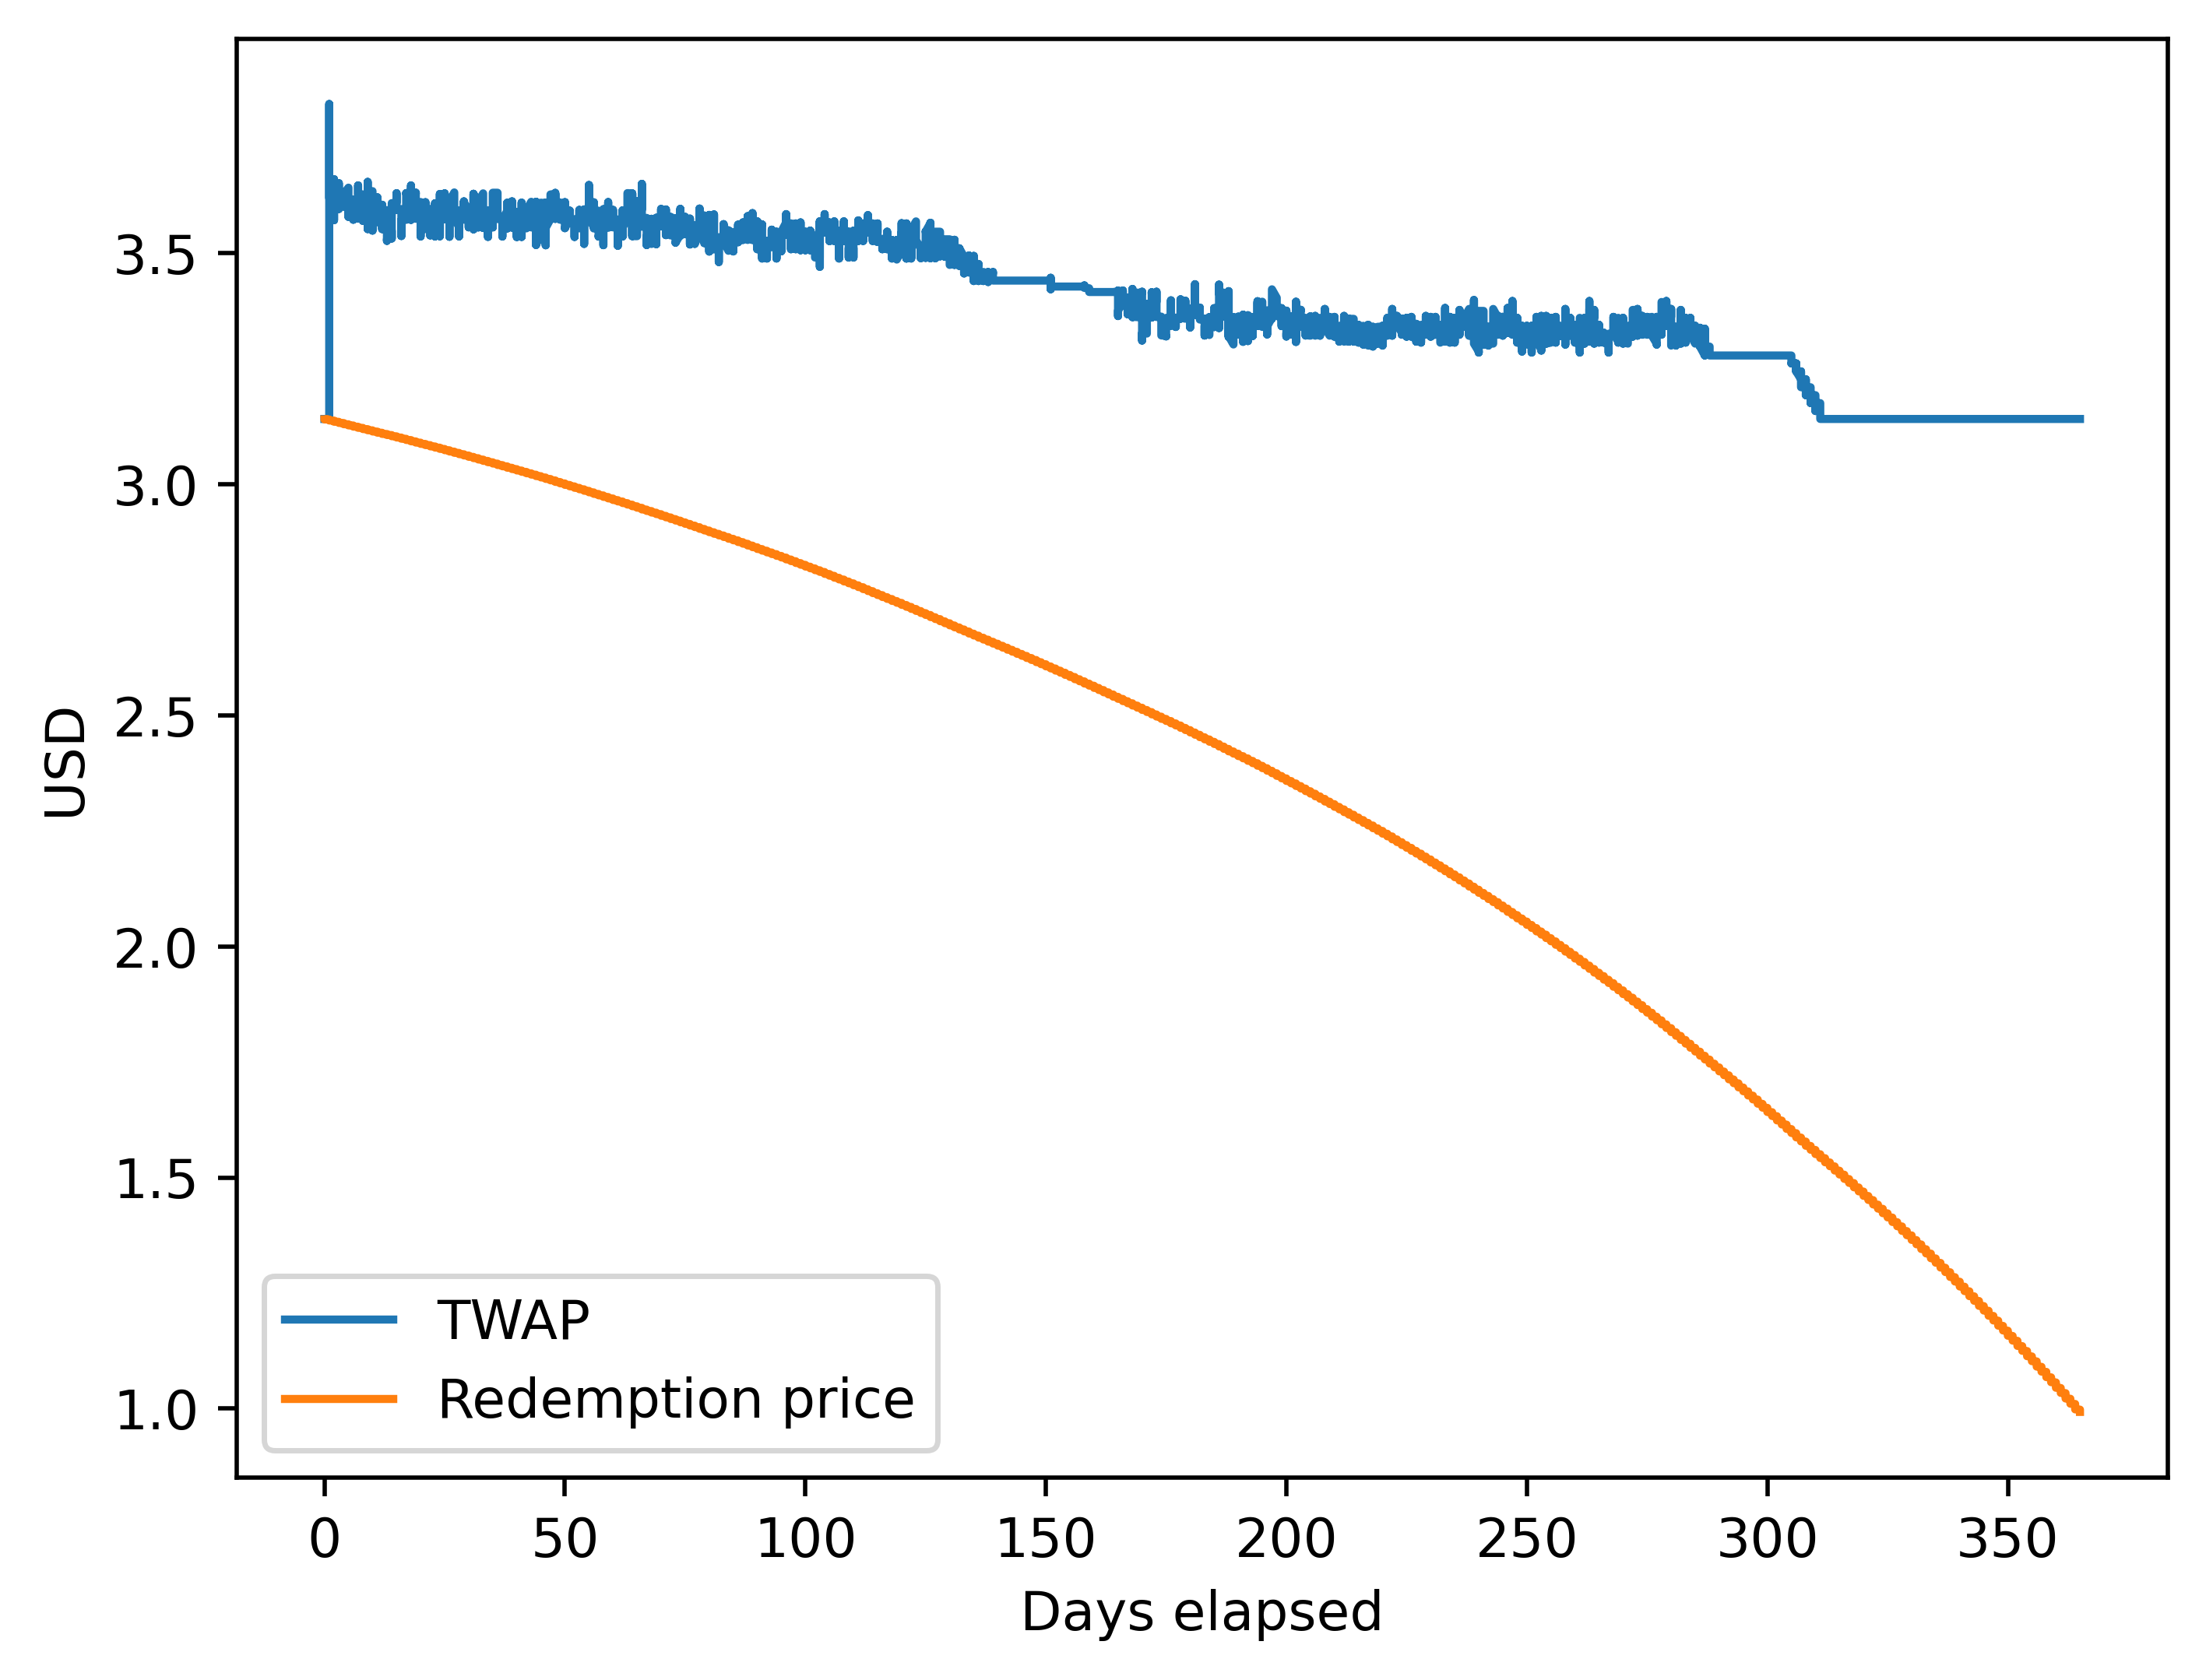
\includegraphics[scale=0.7]{figures/price-evol 2021-03-10 14-34-53.png}
      \end{center}
      \caption{Evolution of the TWAP and redemption price over a year.}
    \end{figure}

    \begin{figure}
      \begin{center}
        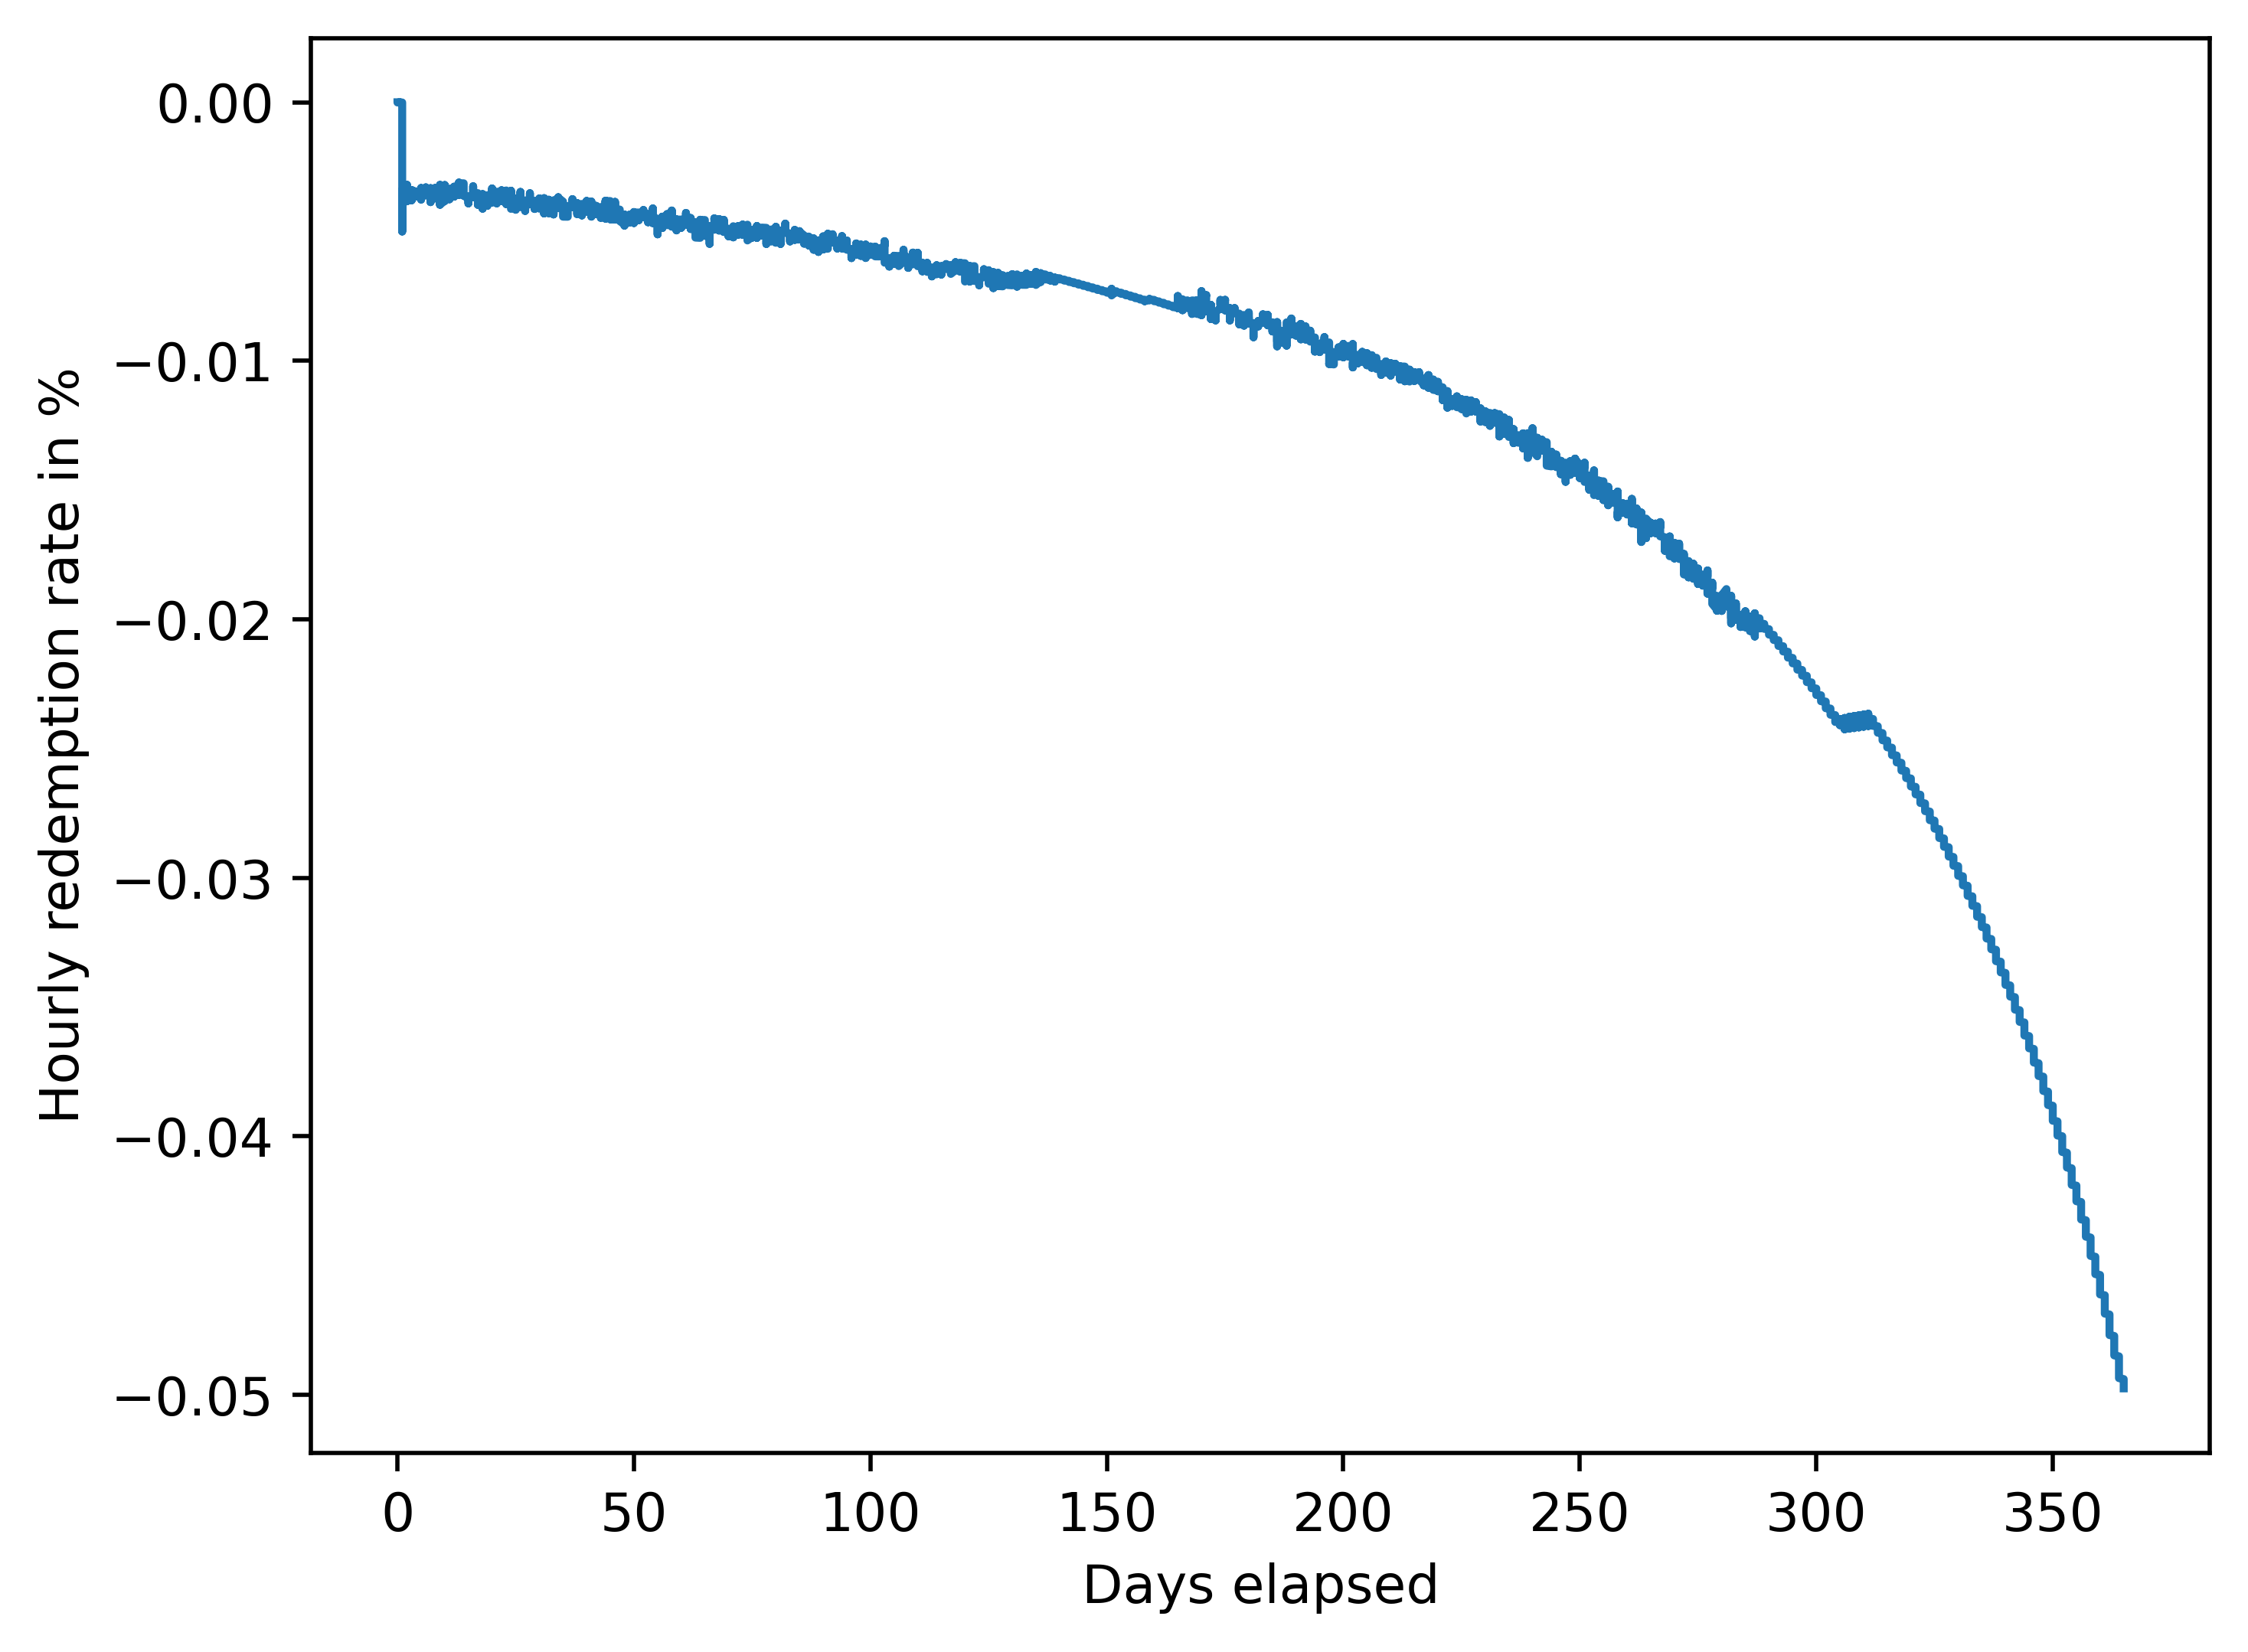
\includegraphics[scale=0.7]{figures/redemption-rate-evol 2021-03-10 14-34-53.png}
      \end{center}
      \caption{Evolution of the hourly redemption rate over a year. The rate increases when the difference between the redemption price and market TWAP decreases and conversely.}
    \end{figure}

    \subsection{Observations}

    From Figure 1, one can develop an intuition of the interaction between the agents and the system and its controller. 
    
    First, the redemption price is equal to the price at which the Uniswap pool is seeded. As a consequence, the error is zero and the only type of return agents have are the positive returns of the liquidity mining rewards. They immediately jump into the pool, moving the price up. 
    
    After 16 hours, the TWAP starts to pick up that change in price, which translates in the RAI controller reading a sudden jump in error and activating the proportional correction. The redemption rate starts to go down, and being negative this translates into a negative expected return that adds to the positive return of the agents. For some agents, this makes their total expected return go below their threshold and makes them drop out of the pool. 

    One surprising feature at first glance is that some agents seem to go in and out of the pool chaotically, instead of dropping sequentially as the returns go below their respective thresholds due to constant decrease of the redemption rate. This can be understood as coupling between the agents. Indeed, the calculation of their returns from liquidity mining depends on their pool share, which in turn depends on the amount of other agents that are in the pool. If a particular agent leaves the pool, this might increase the proportional share of another agent who had previously left it, making their expected return go above threshold again. This musical chair game continues until the redemption rate becomes so low that some agents leave the pool definitely. 
    
    Around day 330 with the parameters of this run, the redemption rate is so low that every agent has left the pool. Since we have seeded the pool with a baseline amount that cannot be withdrawn and that are no other agents capable of driving the market price down in this setup, the price stays exactly the same as the initial price of the pool (constant function market makers are path independent with zero fees), so the error grows indefinitely. 

    In order to confirm the idea of agents expected returns not going down smoothly, the evolution of one particular agents' expected return over the first 50 days is plotted below, as well as the evolution of their pool share.

    \begin{figure}[H]
      \captionsetup[subfigure]{position=b}
      \centering
      \begin{subfigure}[t]{.5\textwidth}
        \centering
        \captionsetup{margin=1.1cm}
        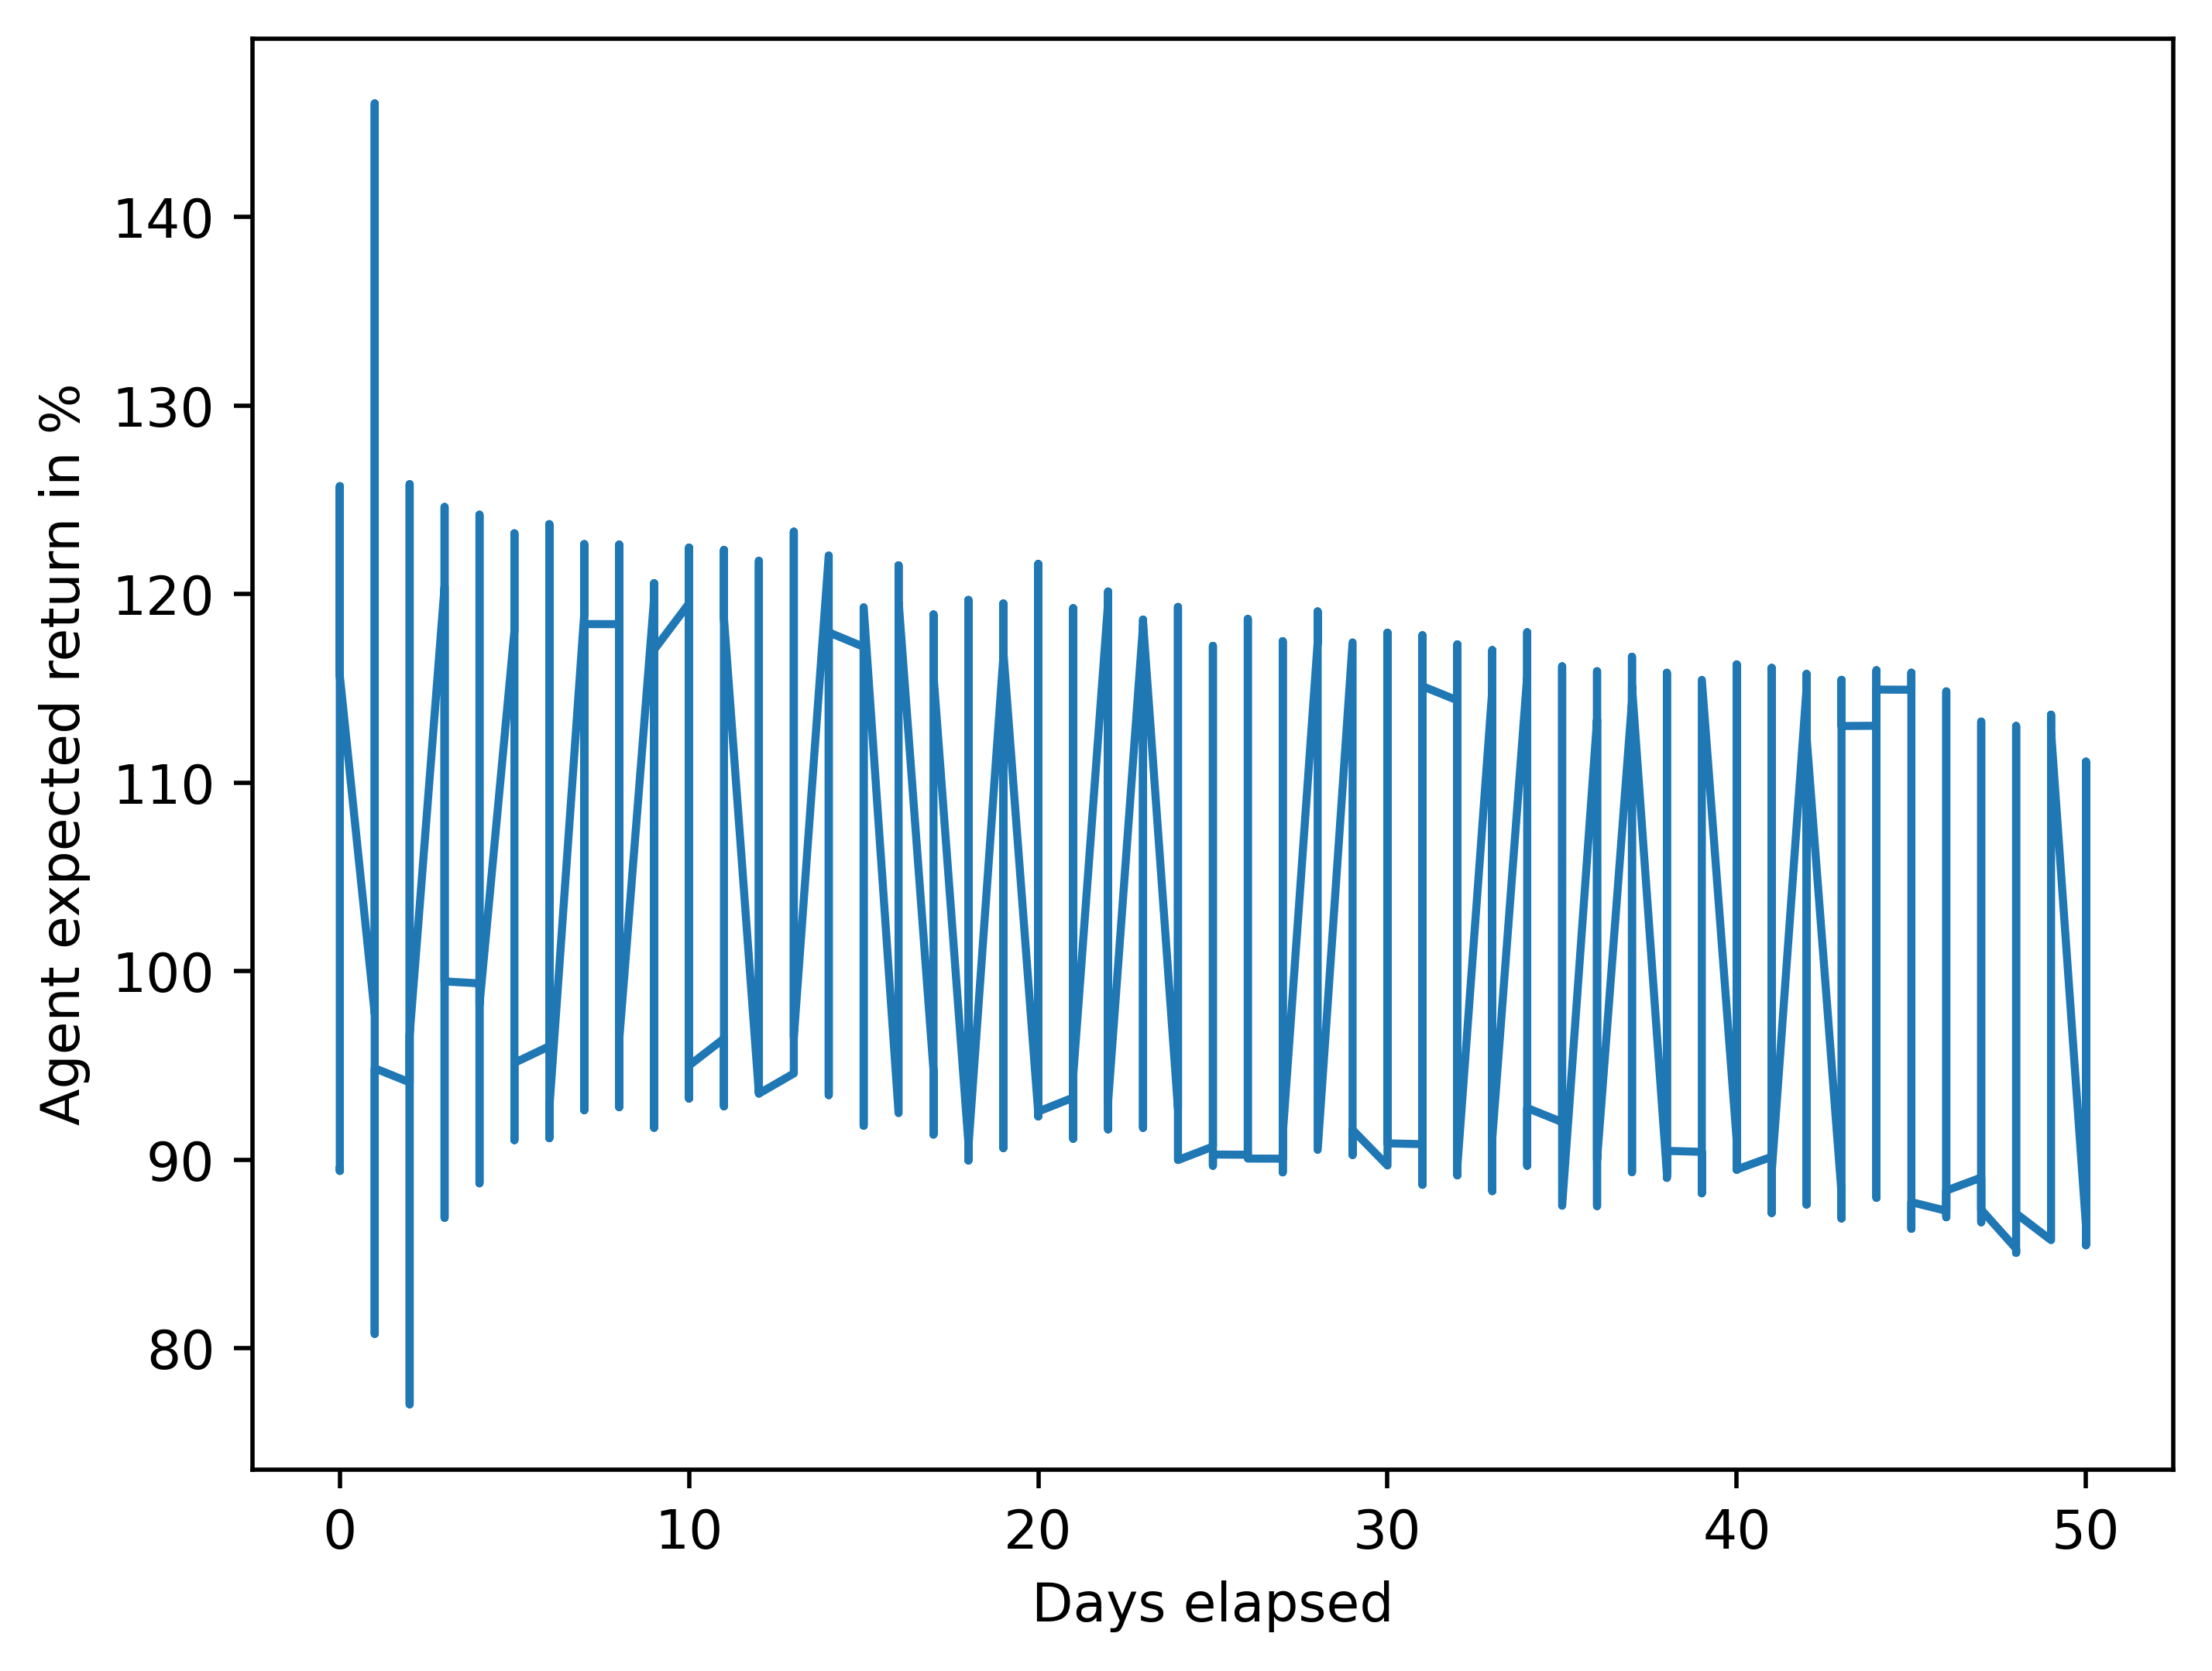
\includegraphics[width=1\linewidth]{figures/agent-return 2021-03-10 15-25-52.png}
        \caption{Evolution of an agent's computed expected return for the first 50 days of the simulation}
      \end{subfigure}%
      \begin{subfigure}[t]{.5\textwidth}
        \centering
        \captionsetup{margin=1.1cm}
        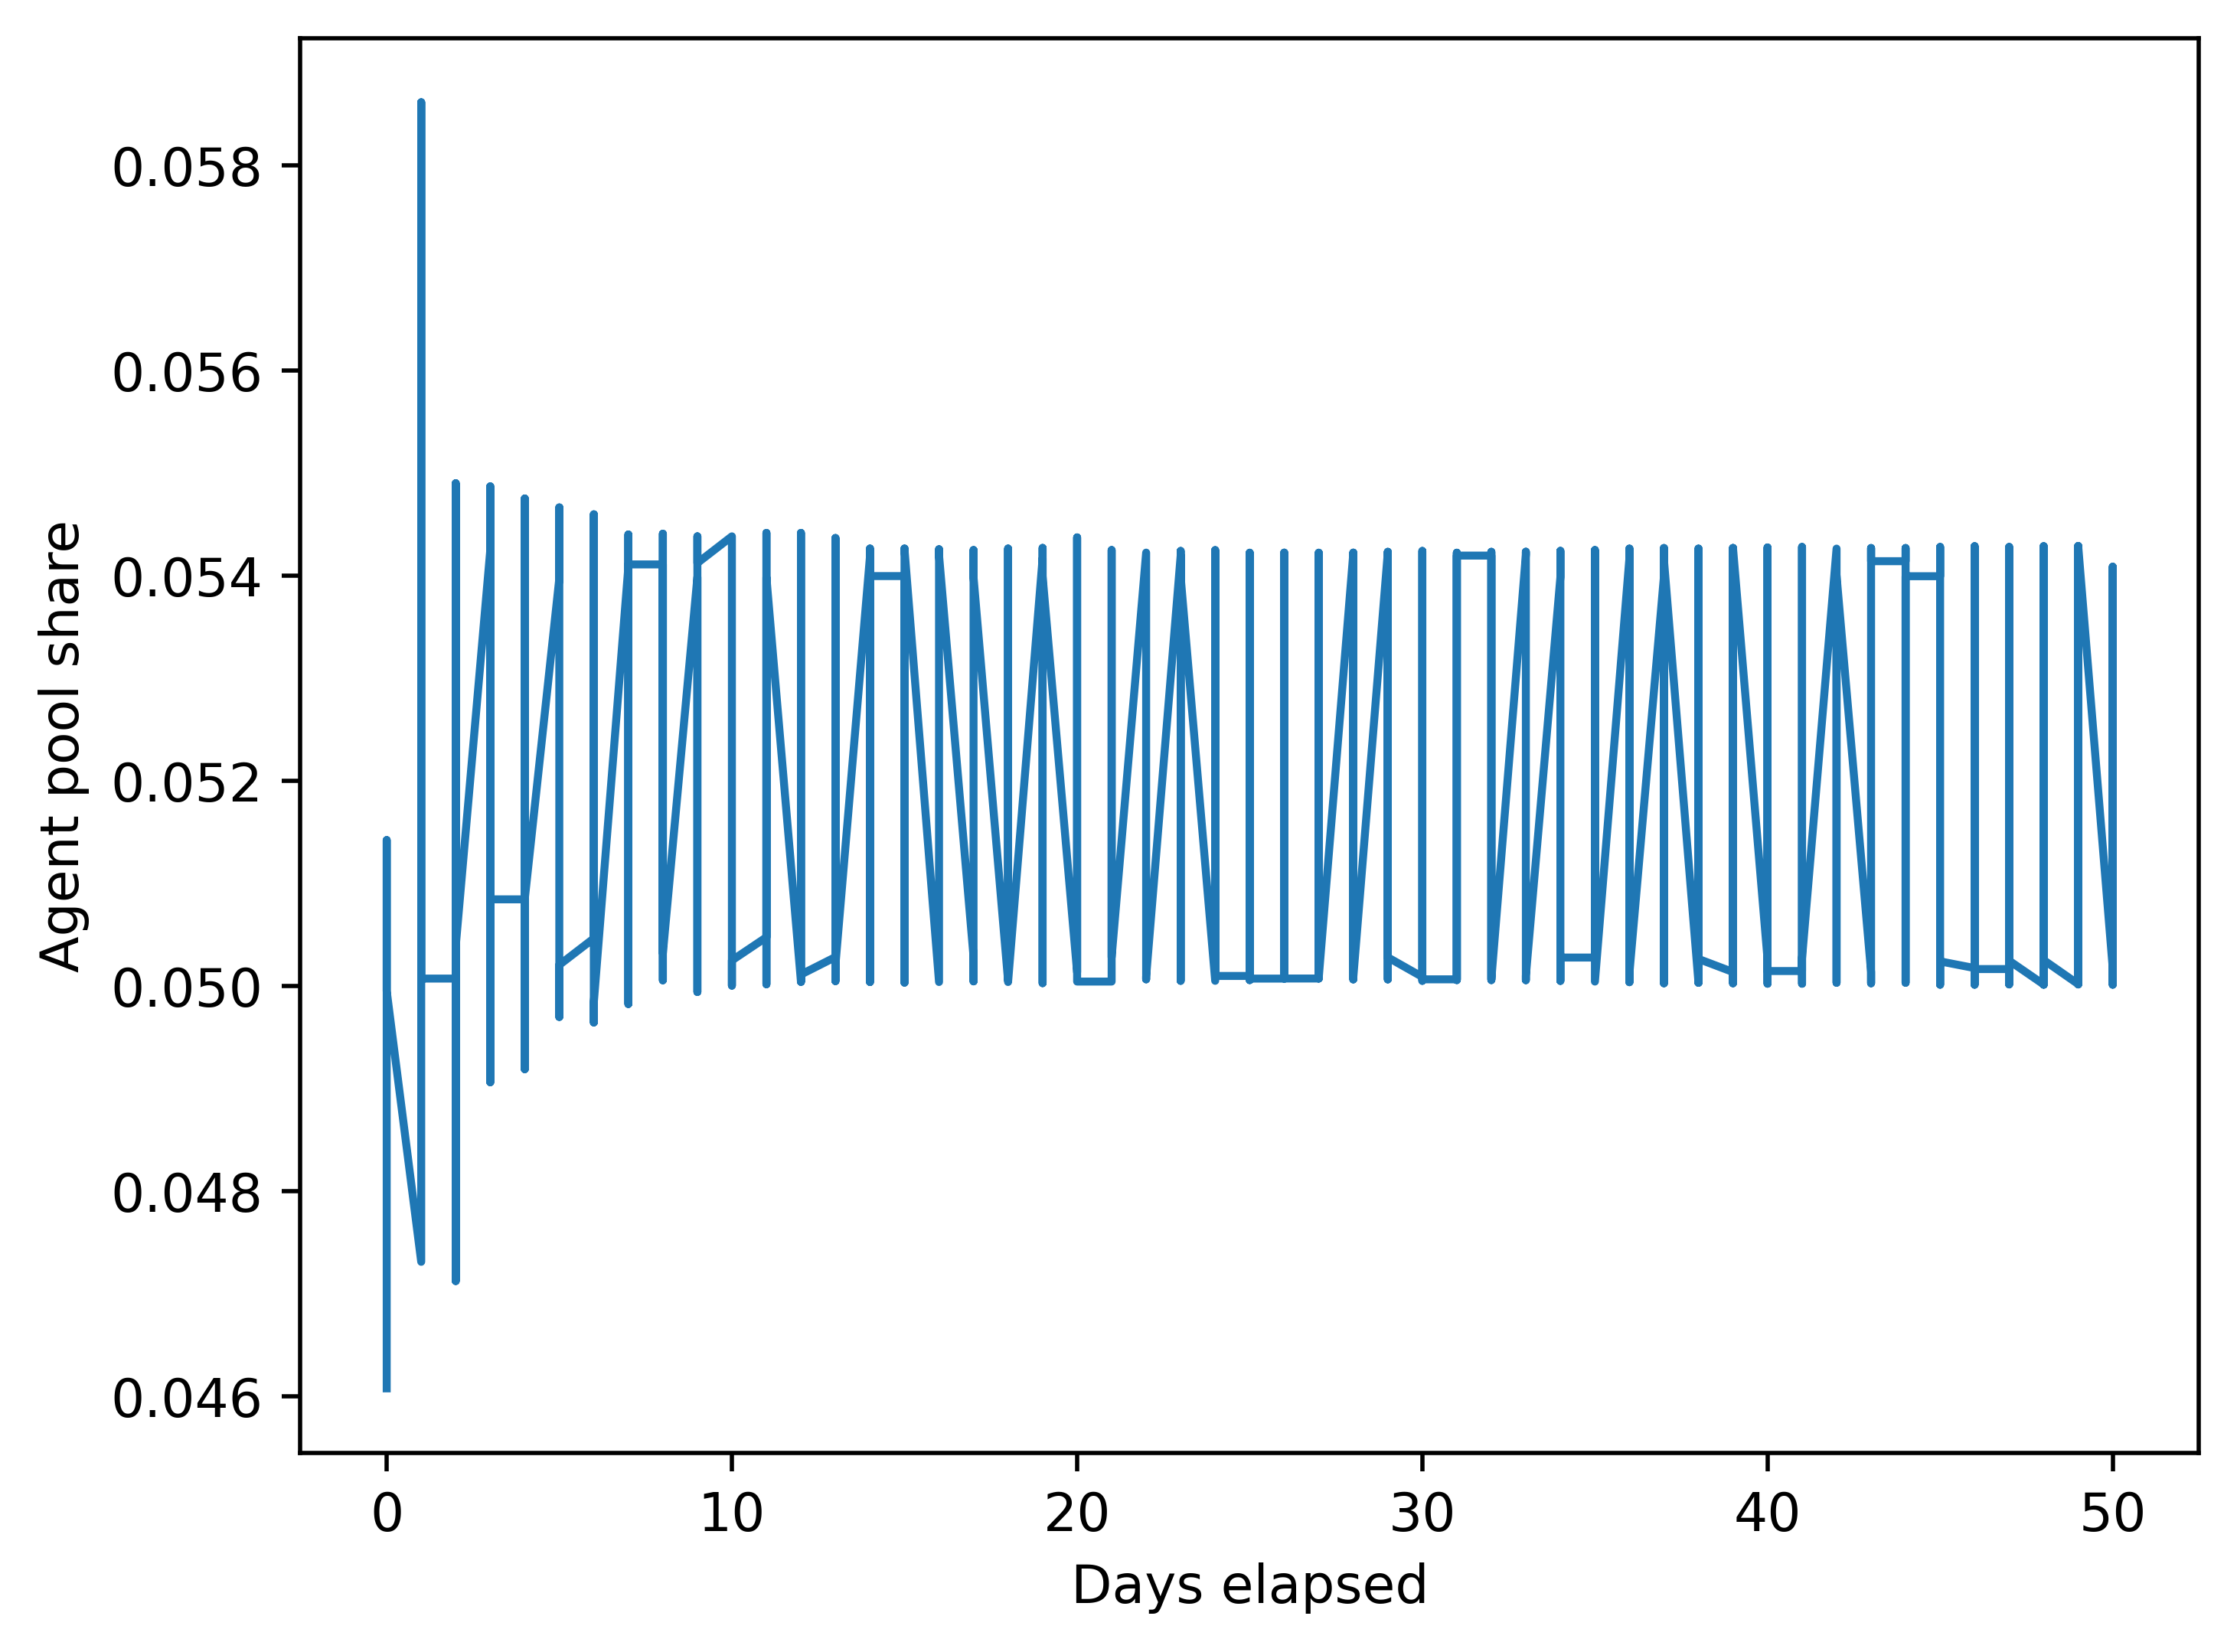
\includegraphics[width=1\linewidth]{figures/agent-pool-share 2021-03-10 15-25-52.png}
        \caption{Evolution of an agent's computed pool share (current, or potential) for the first 50 days of the simulation}
      \end{subfigure}
      \caption{The expected return and pool share of a particular agent are shown to evolve chaotically, as other agents leave and join the pool, their current or potential pool share increases or decreases respectively, influencing their expected return calculations. This coupling explains why the agent's expected returns don't go down setadily with the decreasing redemption rate, and is ultimately the source of the chaotic features of the TWAP evolution.}
    \end{figure}

    While this model is extremely simplistic, some of these observations are likely to remain relevant as more types of agents are added. For example, whether the agents are minting, shorting, buying, etc, there will always exist all kinds of couplings between these different agent types that will make the price action chaotic, which is a general feature of financial markets time series. One could also note that a simple proportional controller is likely to be unstable in many situations. In the simulation setup presented here, it seems that the addition of an integral term would be particularly useful to prevent the divergence.

\end{document}